%%%%%%%%%%%%%%%%%%%% author.tex %%%%%%%%%%%%%%%%%%%%%%%%%%%%%%%%%%%
%
% sample root file for your "contribution" to a proceedings volume
%
% Use this file as a template for your own input.
%
%%%%%%%%%%%%%%%% Springer %%%%%%%%%%%%%%%%%%%%%%%%%%%%%%%%%%


\documentclass{svproc}
%
% RECOMMENDED %%%%%%%%%%%%%%%%%%%%%%%%%%%%%%%%%%%%%%%%%%%%%%%%%%%
%

% to typeset URLs, URIs, and DOIs
\usepackage{url}
\usepackage{amsmath}
\usepackage{algorithm}
\usepackage[noend]{algpseudocode}

\usepackage{graphicx}
%\usepackage{nicefrac}

%\usepackage{caption}
%\usepackage{subcaption}
%\captionsetup{compatibility=false}

% Springer does not support subcaption/caption => use subfig instead and avoid loading the caption package
\usepackage[caption=false]{subfig}


\usepackage{siunitx}
\usepackage{amsmath}
\usepackage{tikz}
\usepackage{adjustbox}

\usepackage{ upgreek }

\usetikzlibrary{arrows, arrows.meta, fit, positioning, quotes,
                shadows, shapes.geometric, shapes.misc}
\usepackage[utf8]{inputenc}

\inputencoding{utf8}



\def\UrlFont{\rmfamily}

%%%%%%%%%%%%% math stuff
\usepackage{amssymb}

%flowchart definitions
\tikzstyle{startstop} = [rectangle, rounded corners, minimum width=3cm, minimum height=1cm,text centered, draw=black, fill=red!30]
\tikzstyle{io} = [trapezium, trapezium left angle=70, trapezium right angle=110, minimum width=3cm, minimum height=1cm, text centered, draw=black, fill=blue!30]
\tikzstyle{process} = [rectangle, minimum width=1cm, minimum height=1cm, text centered, draw=black, fill=white!30]
\tikzstyle{decision} = [diamond, minimum width=1cm, minimum height=1cm, text centered, draw=black, fill=cyan!30]
\tikzstyle{arrow} = [thick,->,>=stealth]

\tikzset{
  font={\fontsize{11pt}{12}\selectfont}}


% vectors in bold
\newcommand{\vp}{\mathbf{p}}
\newcommand{\valpha}{\mathbf{\alpha}}
\newcommand{\vP}{\mathbf{P}}
\newcommand{\vg}{\mathbf{g}}
\newcommand{\vf}{\mathbf{f}}
\newcommand{\vw}{\mathbf{w}}
\newcommand{\vx}{\mathbf{x}}
\newcommand{\vq}{\mathbf{q}}
\newcommand{\vzero}{\mathbf{0}}
\newcommand{\vn}{\mathbf{n}}
\newcommand{\vo}{\mathbf{o}}
\newcommand{\vchi}{\mathbf{\chi}}
\newcommand{\vlbA}{\mathbf{lbA}}
\newcommand{\vubA}{\mathbf{ubA}}
\newcommand{\vlb}{\mathbf{lb}}
\newcommand{\vub}{\mathbf{ub}}


% sets as caligraphics
\newcommand{\cV}{\mathcal{V}}
\newcommand{\cS}{\mathcal{S}}
\newcommand{\cC}{\mathcal{C}}
\newcommand{\cE}{\mathcal{E}}
\newcommand{\cO}{\mathcal{O}}

% misc
\newcommand{\R}{\mathbb{R}} % real numbers

%%%%%%%%%%%%%
\newcommand{\todo}[1]{\textbf{\textcolor{red}{TODO: #1}}}

\begin{document}
\mainmatter              % start of a contribution
%
% Robust Motion Execution
% 
\title{Distributed Real-time Trajectory Replanning for Robust Motion Execution}% in Multi-Robot Systems}


%
%\titlerunning{Distributed Real-time Trajectory Replanning}  % abbreviated title (for running head)
%                                     also used for the TOC unless
%                                     \toctitle is used
%
\author{Baskın Şenbaşlar \and Wolfgang H\"onig \and
Nora Ayanian}
%
%\authorrunning{Ivar Ekeland et al.} % abbreviated author list (for running head)
%
%%%% list of authors for the TOC (use if author list has to be modified)
\tocauthor{Baskın Şenbaşlar, Wolfgang H\"onig, Nora Ayanian}
%
\institute{University of Southern California, Los Angeles CA, USA,\\
\email{\{baskin.senbaslar, whoenig, ayanian\}@usc.edu}}

\maketitle              % typeset the title of the contribution

\begin{abstract}
We propose robust motion execution as a framework that takes pre-planned trajectories as input and compensates for a variety of dynamic changes, including newly appearing obstacles, robots breaking down, or external disturbances.
Robots do not communicate with each other and only sense other robots' positions and the obstacles around them.
At the low-level, we use buffered Voronoi cells as multi-robot collision avoidance strategy.
At the high-level we use a hybrid planning strategy employing both discrete planning and trajectory optimization with a dynamic receding horizon approach.
The discrete planner helps to avoid local minima effectively, adjusts the planning horizon, and provides good initial guesses for the optimization stage.
Trajectory optimization uses a quadratic programming formulation, where all safety-critical parts are formulated as hard constraints.
We demonstrate our approach in simulation and on real robots, showing that it can operate in real-time.
%\keywords{trajectory planning, collision avoidance, multi-robot systems}
\end{abstract}


\section{Introduction}
Motion planning for multi-robot systems is widely used and in particular important in cases where many robots have to interact with each other in confined spaces, potentially with many obstacles around.
Examples include coordination of robots in warehouses~\cite{Kiva}, traffic management at intersections~\cite{IntersectionManagementDresner}, and airport management~\cite{AirportTug}.
Modern planning algorithms can find trajectories that effectively coordinate hundreds of robots while approximately optimizing objectives like total energy used~\cite{crazyplanning-ieeetro}.
All such solutions assume that the resulting trajectories can be executed approximately perfectly, which is not true for teams of hundreds of robots that have to operate persistently.

We propose robust motion execution as a framework that takes pre-planned trajectories as input and compensates for a variety of dynamic changes, including imperfect motion execution of some robots, newly appearing obstacles, robots breaking down, or external disturbances.
Consider the example in Fig.~\ref{fig:swap2}, where two robots are tasked with swapping their positions.
The pre-planned trajectories are collision-free, but neither considers the new obstacle nor that the fact that blue robot does not start at its correct location.
Robust motion execution can be used to successfully swap positions, while staying as close as possible to the pre-planned trajectories.
Our framework is fully distributed and requires no communication; the robots only need to know their own trajectories and need to be able to sense their neighbors' positions and the obstacles around them.

\begin{figure}
%\centering
%\subfloat[Initial configuration and pre-planned trajectories.]{
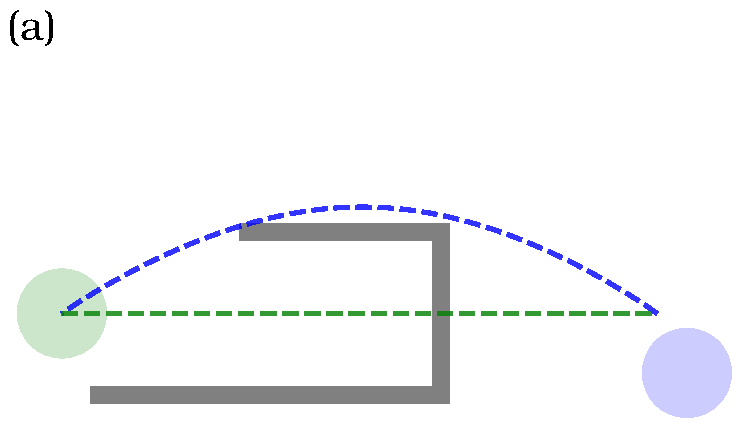
\includegraphics[width=0.45\textwidth]{images/swap2_initial.pdf}
%\label{fig:swap2:initial}
%}
\hfill
%\subfloat[Final configuration and executed trajectories.]{
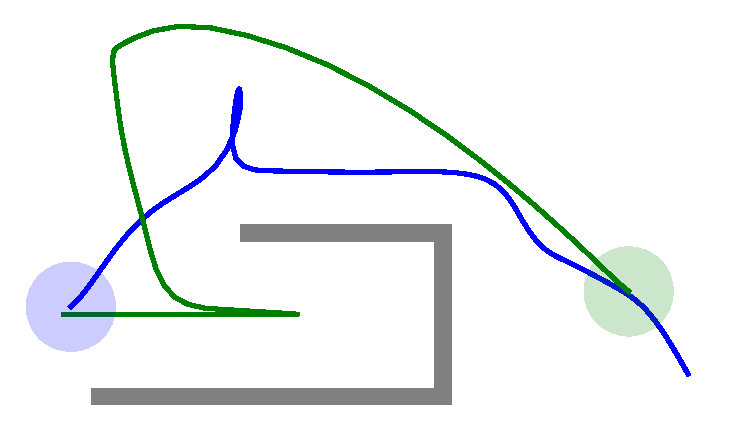
\includegraphics[width=0.45\textwidth]{images/swap2_final.pdf}
%\label{fig:swap2:final}
%}
%\begin{subfigure}[t]{0.48\textwidth}
%\centering
%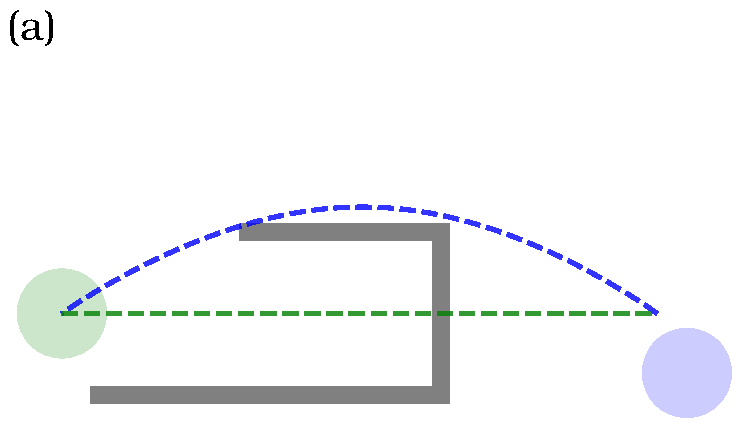
\includegraphics[width=1.0\textwidth]{images/swap2_initial.pdf}
%\caption{Initial configuration.}
%\label{fig:swap2:initial}
%\end{subfigure} \hfill
%\begin{subfigure}[t]{0.48\textwidth}
%\centering
%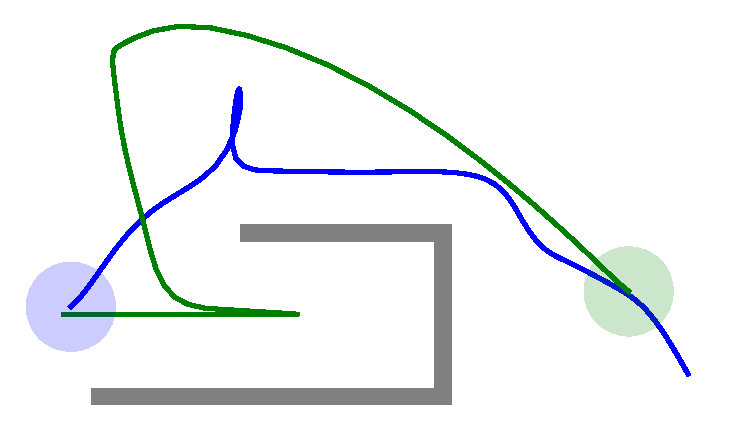
\includegraphics[width=1.0\textwidth]{images/swap2_final.pdf}
%\caption{Final configuration and executed trajectories.}
%\label{fig:swap2:final}
%\end{subfigure}
\caption{Two robots (green and blue circles) are tasked with following their pre-planned trajectories (green and blue dashed lines; (a)).
The initial plans were created without knowledge of the obstacle (gray) and the blue robot does not start at its planned start position.
Our approach computes smooth trajectories in real-time, avoiding the new obstacle and other robots while staying close to the pre-planned trajectory (b).
}
\label{fig:swap2}
\end{figure}

Robust motion execution is an extension of cooperative collision avoidance where the objective is to stay close to the originally planned trajectories as much as possible.
In contrast, traditional collision avoidance methods frequently only take a desired velocity, desired goal state, or desired action as input (see Section~\ref{sec:relatedWork}).
Our method is based on \emph{Buffered Voronoi Cells} (BVC)~\cite{bufferedVoronoiCells} as the underlying cooperative collision avoidance strategy and retains the same theoretical guarantees.
At the high-level we employ a novel combination of trajectory optimization and discrete search-based planning with a dynamic receding horizon approach.
The discrete search allows us to avoid local minima effectively even in difficult scenarios, while the trajectory optimization takes the dynamics of real physical robots into account.



%\todo{perhaps write some more about what experiments we did, after we have the material}

\section{Problem Formulation} \label{problemFormulation}
% assumptions: circular robots; robots follow the same rules; static (or slow) obstacles
% input: original curves; positions of peers; dynamic limits; environment (at least able to sense); dt; curve_count; T
% output: at each dt: new trajectory such that there is no collision (guaranteed)
% issues: no live-lock guarantee

We consider a group of $m$ robots and each robot $i$ is given the following:
\begin{align*}
    \vo_i(t)&:\text{ original trajectory of $i^{th}$ robot where } t\in[0,T_i],\\
    %ct&:\text{ current global time},\\
    %\delta t&:\text{ replanning period},\\
    %\tau&: \text{time horizon},\\ 
    c&:\text{ derivative up to which smoothness is required},\\
    %\cO&:\text{ free space representation of the environment},\\
    %\{\vp_i\}&:\text{ set of positions of all robots},\\
    R_i(\vp)&:\text{ physical extent of robot $i$ at position $\vp$, and}\\
    \gamma_j&: \text{ dynamic limit of the robot for $j^{th}$ derivation degree}.%\\
    %&\ \ \ \ \gamma_j \text{ being the limit for $j^{th}$ derivation degree}\\
\end{align*}

At time $t$, each robot $i$ can sense the positions $\{\vp_1(t),\ldots,\vp_m(t)\}$ of its neighbors as well as the current occupied space $\cO(t)$ around it.
We assume that $\cO(t)$ is a set of $\uptheta$ convex obstacles, which can be achieved in practice by using data structures such as an OctoMap~\cite{octomap}.
Robots cannot communicate with each other and are unaware of the other robots' trajectories.
%Each robot can sense the position of their neighbors, but robots cannot communicate with each other.
Each robot $i$ needs to execute a trajectory $\vf_i(t)$ where $\vf_i(t)$ is a solution to the following optimization problem:
\begin{align}
\begin{split}
    \text{minimize } & \int_{0}^{T_i}\left\|\vf_i(t)-\vo_i(t)\right\|^2 dt\\
    \text{subject to }& \\
    &\vf_i(t) \text{ is}\text{ continuous up to degree $c$},\\
    &\frac{d^j\vf_i}{dt^j}(0) = \frac{d^j\vp_i}{dt^j}(0)\text{ for } j\in\{0,1,...,c\}\\
    &\vf_i(t)\text{ is collision free, and}\\ 
    &\left\|\frac{d^j \vf_i(t)}{dt^j}\right\| \leq \gamma_j\text{ for all desired $j$s},\\
    \text{where } & t\in [0,T_i].
\end{split}
\label{eq:problem:opt}
\end{align}

We approximately solve this problem iteratively using a dynamic receding horizon approach.
At every iteration $K$, robot $i$ plans a trajectory $\vf^{K}_i(t)$ that starts at the robots' current position and is safe to execute up to period $\delta t$.
%We adjust the planning horizon of $\vf^{K}_i(t)$ dynamically to avoid local minima.

%\todo{add paragraph about how we actually (approximately solve this problem)}

% \begin{align*}
%     \text{Given,}\ \ \ \ \ &\\
%     \vo^i(t')&:\text{ original trajectory of robot $i$},\\
%     ct&:\text{ current global time},\\
%     \delta t&:\text{ replanning period},\\
%     \tau&: \text{time horizon},\\ 
%     c&:\text{ maximum continuity between pieces},\\
%     \cO&:\text{ free space representation of the environment},\\
%     \{\vp_i\}&:\text{ set of positions of all robots},\\
%     \gamma&: \text{ dynamic limits of robots in any derivation degree},\\
%     &\ \ \ \ \gamma_j \text{ being the limit for $j^{th}$ derivation degree}\\
%     \text{find a new}&\text{ trajectory $\vf^{i,K}(t)$ such that},\\
%     \vf^{i,K}(t)&\text{ is}\text{ continuous up to degree $c$ for }t\in [0,\tau],\\
%     \frac{d^j\vf^{i,K}}{dt^j}(0) &= \frac{d^j\vf^{i,K-1}}{dt^j}(\delta t)\text{ for } j\in\{0,1,...,c\}\\
%     \vf^{i,K}(t)&\text{ is collision free for $t\in [0,\delta t]$},\\
%     \vf^{i,K}(t)&\text{ tracks $\vo^i(t')$ as close as possible for $t\in[0,\tau]$ or equivalently $t'\in[ct, ct+\tau]$ }, \text{and}\\
%     \left\|\frac{d^j \vf^{i,K}(t)}{dt^j}\right\| &\leq \gamma_j\text{ for } t\in [0,\tau],\\
% \end{align*}



\section{Preliminaries}

We now introduce important mathematical concepts and notations we use.

\subsection{Buffered Voronoi Cells} \label{bufferedVoronoi}
Given a set of $m$ robots with positions $\vp_1,\vp_2,\ldots,\vp_m \in \R^n$ and radii $r_1,r_2,...r_m \in \R$, the buffered Voronoi cell $\cV_i$ of robot $i$ is defined as~\cite{bufferedVoronoiCells}:
\begin{align}
    \cV_i &= \left\{\vp : \forall_{j\neq i} \frac{\vp_j-\vp_i}{\|\vp_j-\vp_i\|}\cdot \vp - \frac{\vp_j-\vp_i}{\|\vp_j-\vp_i\|}\cdot \frac{\vp_j+\vp_i}{2} + r_i\leq 0 \right\} \label{voronoi_cell_definition}
\end{align}
where $\|\vp\|$ is the L2-norm of vector $\vp$.

The inequality inside \eqref{voronoi_cell_definition} defines a hyperspace $\cS_i^j$ that is bounded by hyperplane $H_i^j$ that separates point $\vp_i$ from $\vp_j$ with normal $\valpha_i^j$ and distance along normal $\beta_i^j$ where $\valpha_i^j\in \R^n$ and $\beta_i^j\in \R$ such that
\begin{equation}
    \valpha_i^j = \frac{\vp_j - \vp_i}{\|\vp_j-\vp_i\|} \text{ and }
    \beta_i^j = \valpha_i^j \cdot \left(\frac{\vp_i + \vp_j}{2}\right) - r_i.
    \label{voronoiAlphaBeta}
\end{equation}
% \begin{align}
%     \valpha_i^j &= \frac{\vp_j - \vp_i}{\|\vp_j-\vp_i\|}\label{voronoiAlpha}\\
%     \beta_i^j &= \valpha_i^j \cdot \left(\frac{\vp_i + \vp_j}{2}\right) - r_i. \label{voronoiBeta}
% \end{align}

% The set of all buffered Voronoi cells is called the buffered Voronoi decomposition of the space.
For a given buffered Voronoi decomposition of the space, any point $\vp\in \R^n$ can be inside at most one of the buffered Voronoi cells.
We use this property in order to avoid robot-to-robot collisions.

Using the hyperspaces $\cS_i^j$ we can reformulate $\cV_i$ as follows:
\begin{equation}
    \cV_i = \bigcap\limits_{j\neq i} \cS_i^j \text{ , where } \cS_i^j = \left\{\vp : \valpha_i^j \cdot \vp - \beta_i^j \leq 0\right\}.
    \label{voronoiEquation}
\end{equation}

% \begin{align}
%     \cS_i^j = \left\{\vp : \valpha_i^j \cdot \vp - \beta_i^j \leq 0\right\}
% \end{align}

% Using this definition, an equivalent definition for the set \eqref{voronoi_cell_definition} is
% \begin{align}
%     \cV_i = \bigcap\limits_{j\neq i} \cS_i^j \label{voronoiEquation}.
% \end{align}

Thus, we can compute the buffered Voronoi cell of any robot $i$ as the set of hyperplanes $H_i^j$ in $O(m)$ time.

\subsection{B\'ezier Curves} \label{bezierCurves}
A degree $d$ B\'ezier curve $\vf(t)$ parametrized by duration $T$ is defined by $d+1$ control points $\vP_0, \vP_1, ..., \vP_d \in \R^n$ such that
\begin{align}
    \vf(t; T) = \sum_{i=0}^d \vP_i {d\choose i}\left(\frac{t}{T}\right)^i\left(1-\frac{t}{T}\right)^{d-i},\hskip .5cm 0\leq t \leq T.
\end{align}

The curve starts at $\vP_0$ and ends at $\vP_d$, however does not interpolate other control points.
A B\'ezier curve lies completely inside the convex hull of its control points~\cite{Bernstein}.
%This is called the \emph{convex hull property of B\'ezier curves}.
We use this property to avoid robot-to-obstacle collisions.

We use splines as trajectories where each piece is a B\'ezier curve. Given a trajectory $\vf^{K}_i(t)$ for robot $i$ with $l$ pieces and duration $T^{K}_i$ at iteration $K$, $T^{K}_{i,j}$ denotes the duration of the $j^{th}$ piece where $j \in \{1,2,\ldots,l\}$. $\vf^{K}_{i,j}(t)$ denotes the $j^{th}$ piece of the trajectory with implicit duration parameter $T^K_{i,j}$ where $t\in[0, T^{K}_{i,j}]$. $\vP^{K}_{i,j,\rho}$ denotes the $\rho^{th}$ control point of the $j^{th}$ piece where $\rho \in \{0,1,\ldots,d\}$.


% \subsection{Support Vector Machine}\label{svmSection}
% A support vector machine is a supervised learning method that is used to classify data into several classes.
% In binary classification problems, we are given a linearly separable data set $\{(\vx_i, y_i)\}$ where $\vx_i \in \R^n$ is a data point and $y_i \in \{-1, 1\}$ is the corresponding class label.
% The goal is to find a hyperplane with normal $\vw$ and distance along the normal $\frac{b}{\|w\|}$ that separates the two classes.
% The SVM problem for binary classification with a separable data set can be stated as the following quadratic optimization problem with hard constraints \cite{SVM}:
% \begin{align*}
%     \text{minimize}\ \ \  &\|\vw\|\\
%     \text{subject to}\ \ \  & y_i(\vw \cdot \vx_i - b) \geq 1
% \end{align*}
% We use SVMs to define collision free convex subspaces that are obstacle-free.

\subsection{Trajectory Optimization using Quadratic Programming} \label{trajectoryOptimization}
A part of our replanning approach utilizes \emph{quadratic programming} (QP) for trajectory optimization.
The decision variables $\vx$ are all B\'ezier curve control points concatenated.
The overall structure of our quadratic optimization problem is as follows:
\begin{align}
\begin{split}
    \text{minimize}\ \ \ &\frac{1}{2}\vx^TH\vx + \vx^T\vg\\
    \text{subject to}\ \ \ & \vlbA \leq A\vx \leq \vubA.
    % &\vlb \leq \vx \leq \vub
\end{split}
\end{align}
%, while bounds on variables are represented with vectors the $\vlb$ and the $\vub$.

A quadratic cost function is represented using the matrix $H$ and the vector $\vg$. The constraints are represented using the matrix $A$ with vectors $\vlbA$ and $\vubA$.
Notice that all constraints should be linear in the decision variables.

There are three types of constraints we impose on the curves: \emph{initial point constraints}, \emph{continuity constraints}, and \emph{hyperspace constraints}.
An initial point constraint on a B\'ezier curve requires the initial point of the curve to be equal to a given vector for a specified derivative. This translates to $n$ linear constraints on control points, $n$ being the dimension we are working in.
A continuity constraint between curve $j$ and curve $j+1$ requires the end of curve $j$ to be equal to the beginning of curve $j+1$ at any order of differentiation.
We take the vector difference of those values and require it to be equal to $\vzero$. This translates to $n$ linear constraints on control points.
A hyperspace constraint requires all control points of a curve to be on a specific side of a hyperplane. If a curve has $d+1$ control points, this translates to $d+1$ constraints on control points. All 3 types of constraints are linear in control points, and the exact construction is discussed in a previous work~\cite{crazyplanning-ieeetro}.

% There are three types of constraints we impose on the curves: \emph{initial point constraints}, \emph{continuity constraints}, and \emph{hyperspace constraints}.

% \begin{description}
% \item [Initial Point Constraints]
% An initial point constraint on a B\'ezier curve requires the first control point of the curve to be equal to a given vector.
% This requires $n$ linear constraints on the control points. %, $n$ being the dimension we are working in.

% \item[Continuity Constraints]
% A continuity constraint between curve $j$ and curve $j+1$ requires curve $j$ at the end to be equal to the curve $j+1$ at the beginning in any order of derivation.
% We take the vector difference of those values and require it to be equal to $\vzero$.
% This requires $n$ linear constraints on the control points.

% \item[Hyperspace Constraints]
% A hyperspace constraint requires all points of a curve to be on a specific side of a hyperplane.
% Given a hyperplane with normal $\vn$ and distance along the normal $b$, the hyperspace constraint requires one linear constraint for each relevant control point.
% \end{description}

% The construction of the QP is discussed in more detail in previous work~\cite{crazyplanning-ieeetro}.

\section{Approach}

% TODO: running example?

%\subsection{Approach Overview}
Replanning is done at a fixed period of $\delta t$ and at each iteration $K$ we compute a trajectory $f^K_i(t)$.
The planning horizon $\tau'$ is automatically adjusted, but the desired planning horizon $\tau$ can be provided.
In the following, we assume that the robots are spherical with a uniform radius $r_s$.
%The trajectory $f^K_i(t)$ is safe to execute at least up to time $\delta t$, and minimizes the deviation from the original trajectory $o_i(t)$.

We execute the following three major components iteratively: \emph{discrete planning} that is used to efficiently plan around new obstacles, \emph{trajectory optimization} to generate smooth and collision-free trajectories, and \emph{temporal rescaling} to enforce the dynamic limits of the robot, see Fig.~\ref{fig:flowchart}.
%In the beginning of each iteration, we check several conditions to decide if discrete planning is required.
%If discrete planning is required, we execute a discrete search that results in a discrete path that is collision free but not smooth.
%We use this discrete path as an initial guess in trajectory optimization.
%If discrete planning is not required, we use the control points of the previous plan as the initial guess.

%We construct a QP with hard constraints for trajectory optimization in a slightly different way depending on whether discrete planning was executed or not.
%In both cases, buffered Voronoi cells are used to ensure collision-free operation for up to time $\delta t$ and collisions with static obstacles are avoided for the planning horizon.

%Dynamic limits cannot be represented as linear constraints in our QP.
%Thus, we check dynamic limit violations in the temporal rescaling stage that runs after optimization.
%As long as dynamic limits are violated, we increase the durations of all trajectory pieces uniformly, followed by re-solving of the QP.

%At the end of each iteration, each robot has its trajectory $\vf^{K}_i(t)$ that is guaranteed to be collision-free up to time $\delta t$, is continuous up to the $c^{th}$ derivative, obeys the dynamic limits of the robot, tries to stay close to the original trajectory, and is a good starting point for the next iteration. We execute this trajectory for a period of $\delta t$ and replan for the next iteration.

\begin{figure}
\centering
%\begin{adjustbox}{width=\textwidth,caption={bla}}
\resizebox{0.9\textwidth}{!}{
% \footnotesize
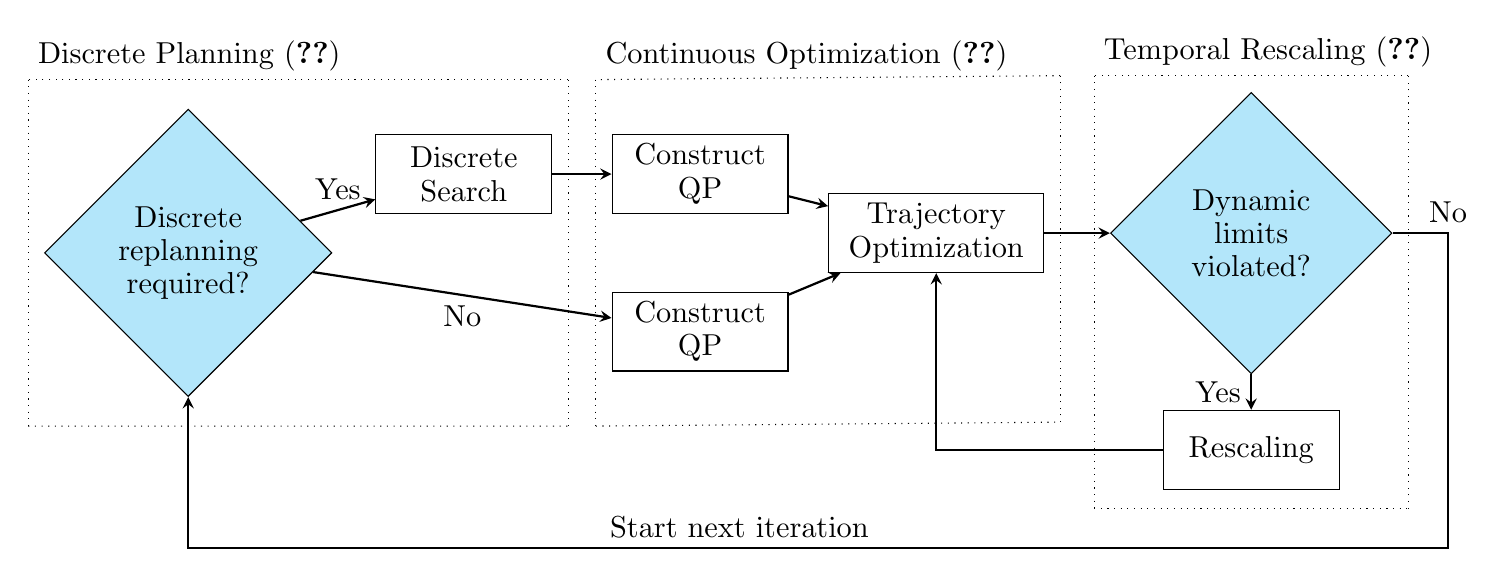
\begin{tikzpicture}[node distance = 2cm]
    \node (discrete) [decision, text width=2cm] {Discrete replanning required?};
    \node (discretesearch) [process, right of=discrete, xshift=1.5cm, yshift = 1cm, text width = 2cm] {Discrete Search};
    \node (discobjbuild) [process, right of=discretesearch, xshift = 1cm, text width = 2cm] {Construct QP};
    \node (contobjbuild) [process, below of=discobjbuild, text width = 2cm] {Construct QP};
    %\node (constraintbuild) [process, right of=discobjbuild, yshift = -0.75cm, xshift = 1cm, text width=2cm]
    %{constraint builder};
    \node (trajopt) [process, right of=discobjbuild, yshift = -0.75cm, xshift = 1cm, text width = 2.5cm] {Trajectory Optimization};
    \node (dynamiclimits) [decision, right of=trajopt, xshift = 2.0cm, text width = 2cm] {Dynamic limits violated?};
    \node (rescale) [process, below of = dynamiclimits, text width = 2cm, yshift = -0.75cm] {Rescaling};
    %\node (end) [io, right of = dynamiclimits, text width = 2cm, xshift = 2.5cm] {use trajectory for $\delta t$};
    
    \coordinate[above=2cm of discrete.west, xshift=-0.2cm, yshift=0.2cm] (c1);
    \coordinate[below=2cm of discrete.west, xshift=-0.2cm, yshift=-0.2cm] (c2);
    \coordinate[above=2cm of discretesearch.east, xshift = 0.2cm, yshift=-0.8cm] (c3);
    \coordinate[below=2cm of discretesearch.east, xshift = 0.2cm, yshift = -1.2cm] (c4);
    
    
    \coordinate[above=2cm of discobjbuild.west, xshift=-0.2cm, yshift=-0.8cm] (c5);
    \coordinate[below=2cm of discobjbuild.west, xshift=-0.2cm, yshift = -1.2cm] (c6);
    \coordinate[above=2cm of trajopt.east, xshift = 0.2cm] (c7);
    \coordinate[below=2cm of trajopt.east, xshift = 0.2cm, yshift=-0.4cm] (c8);
    
    
    \coordinate[above=2cm of dynamiclimits.west, xshift=-0.2cm] (c9);
    \coordinate[below=2cm of dynamiclimits.west, xshift=-0.2cm, yshift = -1.5cm] (c10);
    \coordinate[above=2cm of dynamiclimits.east, xshift = 0.2cm] (c11);
    \coordinate[below=2cm of dynamiclimits.east, xshift = 0.2cm, yshift = -1.5cm] (c12);
    
    \draw [arrow] (discrete) -- node[anchor=south] {Yes} (discretesearch);
    \draw [arrow] (discrete) -- node[anchor=north] {No} (contobjbuild);
    \draw [arrow] (discretesearch) -- (discobjbuild);
    \draw [arrow] (discobjbuild) -- (trajopt);
    \draw [arrow] (contobjbuild) -- (trajopt);
    %\draw [arrow] (constraintbuild) -- (trajopt);
    \draw [arrow] (trajopt) -- (dynamiclimits);
    \draw [arrow] (dynamiclimits) -- ++(2.5,0) node[anchor=south] {No} -- ++(0,-4) --  ++(-5,0) -- ++(-4,0) node[anchor=south] {Start next iteration} -|   (discrete);
    \draw [arrow] (dynamiclimits) -- node[anchor=east] {Yes} (rescale);
    \draw [arrow] (rescale) -| (trajopt);
    
    \node[right = 0cm of c1, yshift=0.3cm] {Discrete Planning (\ref{discretePlanning})};
    \node[right = 0cm of c5, yshift=0.3cm] {Continuous Optimization (\ref{continuousOptimization})};
    \node[right = 0cm of c9, yshift=0.3cm] {Temporal Rescaling (\ref{temporalRescaling})};
    
    \draw [dotted] (c1) -- (c2);
    \draw [dotted] (c2) -- (c4);
    \draw [dotted] (c4) -- (c3);
    \draw [dotted] (c3) -- (c1);
    
    \draw [dotted] (c5) -- (c6);
    \draw [dotted] (c6) -- (c8);
    \draw [dotted] (c8) -- (c7);
    \draw [dotted] (c7) -- (c5);
    
    
    \draw [dotted] (c9) -- (c10);
    \draw [dotted] (c10) -- (c12);
    \draw [dotted] (c12) -- (c11);
    \draw [dotted] (c11) -- (c9);
\end{tikzpicture}
}
%\end{adjustbox}
\caption{Overview of the replanning pipeline.
}
\label{fig:flowchart}
\end{figure}

%\todo{DISCUSS: planning/execution overlap?}

\subsection{Discrete Planning} \label{discretePlanning}

In each planning iteration $K$ that corresponds to the current time $\psi$, we sense the neighbors' positions and compute the buffered Voronoi cell $\cV_i(\psi)$.
We also assume that we have a current representation of the occupied space ($\cO(\psi)$), which can be achieved in practice by using LIDAR or RGB-D sensors.

Robot $i$ executes discrete planning if any of the following conditions are true:
\begin{enumerate}
    \item The original trajectory is not collision-free for the desired time horizon $\tau$, i.e., $\exists t\in [\psi,\psi+\tau] : R_i(\vo_i(t)) \cap \cO(\psi) \neq \emptyset$,
    \item The first piece of the previously planned trajectory is outside the robot's buffered Voronoi cell, i.e., $\exists t\in [0, T^{K-1}_{i,1}] : \vf^{K-1}_{i,1}(t) \not\in \cV_i(\psi)$, or
    \item The previously planned trajectory is not collision-free for the desired time horizon $\tau$, i.e., $\exists t\in [0,\tau] :  R_i(\vf^{K-1}_i(t)) \cap \cO(\psi) \neq \emptyset$.
\end{enumerate}
The first condition handles cases where previously unknown obstacles block the pre-planned path of a robot, the second case handles cases where previously unknown robots appear and robots move towards each other a lot, and the third condition handles numeric issues and dynamic obstacles.

Discrete planning uses a dynamic receding horizon approach. First, we find the earliest time $\tau'\in [\min(\tau, T_i-\psi), T_i-\psi]$ where the original trajectory is collision-free at time $\psi + \tau'$ with respect to both obstacles and other robots.
Second, we use a discrete graph search to find a path from the robots current location to $\vo_i(\psi+\tau')$ that avoids both static obstacles and other robots.
If $\tau'$ does not exist or no solution path exists, we skip the discrete planning stage and construct QP as if discrete planning was not required.
Third, we use the first $l$ segments of the discrete path to uniformly place the new estimated control points on top of those segments.
In case the discrete path has fewer than $l$ segments, the last discrete segment is shared between multiple B\'ezier curves.
Finally, we adjust $T_{i,j}^K$ relative to the segment lengths and scale by $\tau'$, such that we would arrive at time $\psi+\tau'$ at $\vo_i(\psi+\tau')$ if we followed the discrete path with constant speed.
To guarantee collision-free operation, we ensure that $T_{i,1}^K\geq \delta t$ in any case.

An example is shown in Fig.~\ref{fig:swap2_2} (a). 
Discrete planning is executed because the original trajectory (green dashed line) passes through an obstacle.
The earliest time to avoid the obstacle $\tau'$ is found such that the green robot re-joins its original trajectory after the obstacle.
A path that avoids both the static obstacle and the other (blue) robot is found (green dotted line) and has a total of six path segments.
The first four ($l=4$) segments are used to place new guesses of B\'ezier control points (blue, green, red, and cyan circles).
In this example, each curve has eight control points, although some of the points overlap.
The duration for each B\'ezier curve $T^{K}_{i,j}$ is adjusted according to the path length; for example, the duration of the segment with the red control points ($T_{i,3}^K$) is approximately twice as long as the duration of the segment with the green control points ($T_{i,2}^K$).

\begin{figure}
\centering
%\subfloat[Discrete path around an obstacle and other robot back to the original trajectory.]{
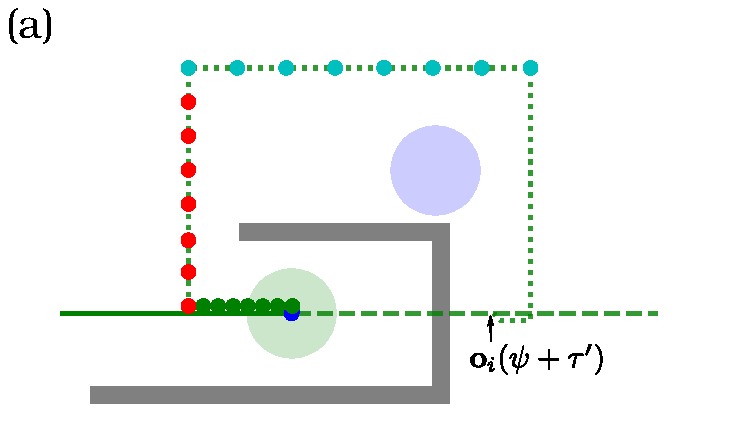
\includegraphics[width=0.45\textwidth]{images/swap2_discrete.pdf}
%\label{fig:swap2:discrete}
%}
\hfill
%\subfloat[Continuous trajectory split into four pieces and respective hyperspaces.]{
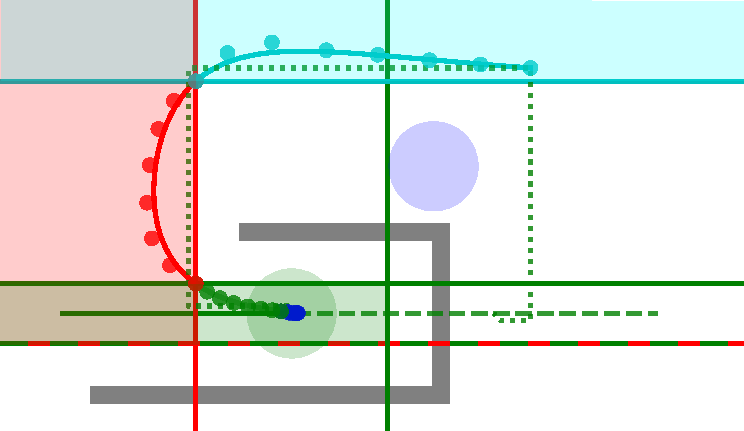
\includegraphics[width=0.45\textwidth]{images/swap2_cont_red.pdf}
%\label{fig:swap2:cont}
%}
% \begin{subfigure}[t]{0.48\textwidth}
% \centering
% 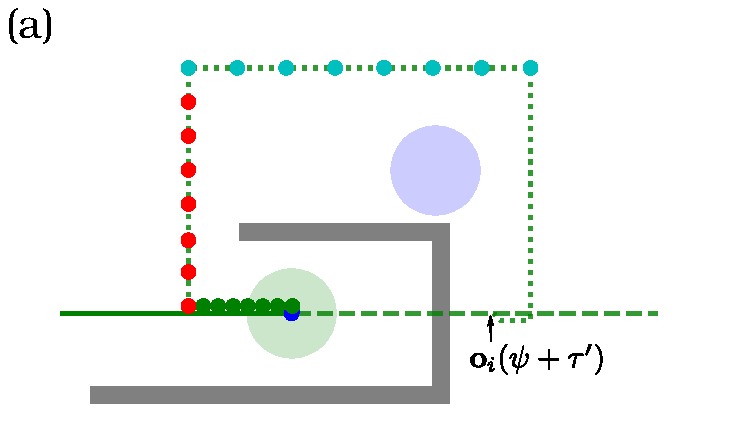
\includegraphics[width=1.0\textwidth]{images/swap2_discrete.pdf}
% \caption{Discrete path around an obstacle and other robot back to the original trajectory.}
% \label{fig:swap2:discrete}
% \end{subfigure} \hfill
% \begin{subfigure}[t]{0.48\textwidth}
% \centering
% 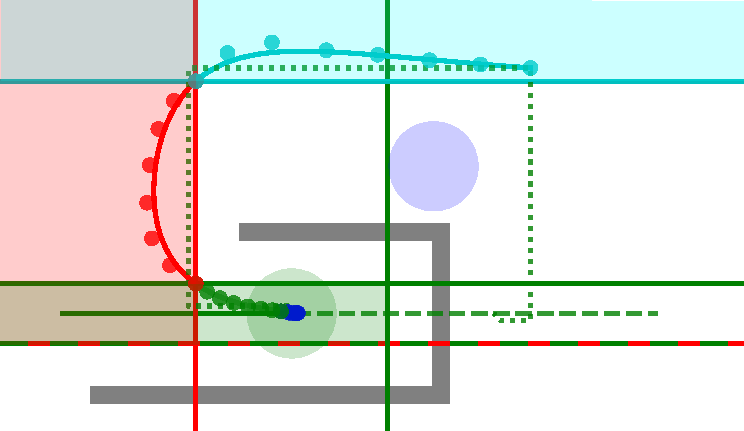
\includegraphics[width=1.0\textwidth]{images/swap2_cont_red.pdf}
% \caption{Continuous trajectory split into four pieces and respective hyperspaces.}
% \label{fig:swap2:cont}
% \end{subfigure}
\caption{
Example at $t=\SI{3.9}{s}$.
Discrete path around an obstacle and other robot back to the original trajectory (a).
Continuous trajectory split into four pieces and respective hyperspaces (b).
}
\label{fig:swap2_2}
\end{figure}

% \begin{figure}
% \centering
% \subfloat[Voronoi decomposition.]{
% 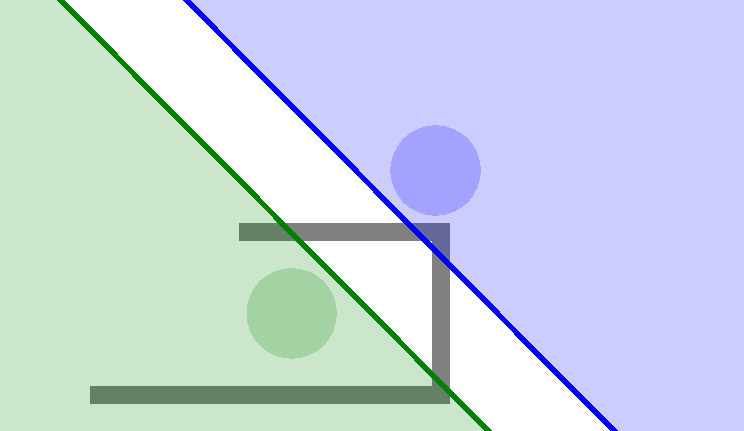
\includegraphics[width=0.48\textwidth]{images/swap2_voronoi.pdf}
% \label{fig:swap2:voronoi}
% }
% % \begin{subfigure}[b]{0.48\textwidth}
% % \centering
% % 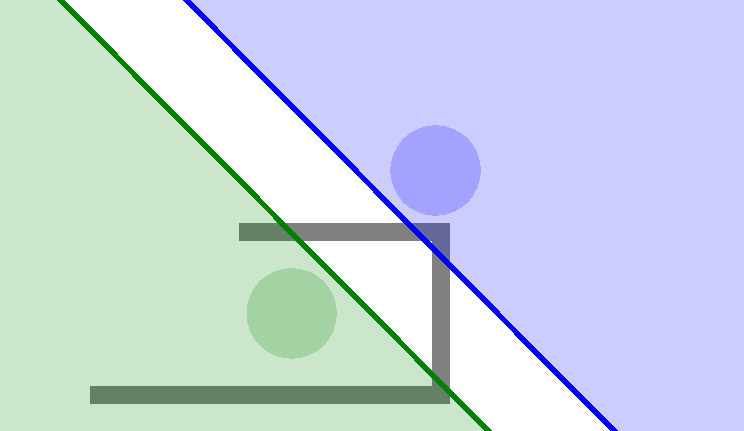
\includegraphics[width=1.0\textwidth]{images/swap2_voronoi.pdf}
% % \caption{Voronoi decomposition.}
% % \label{fig:swap2:voronoi}
% % \end{subfigure} \hfill
% % \begin{subfigure}[b]{0.45\textwidth}
% % \centering
% % 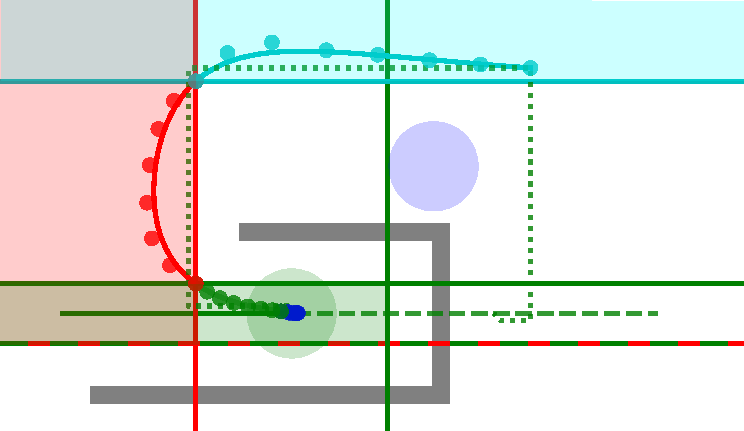
\includegraphics[scale=0.6]{images/swap2_cont_red.pdf}
% % \caption{Continuous trajectory split into four pieces and respective hyperspaces.}
% % \label{fig:swap2:cont}
% % \end{subfigure}
% \caption{
% %Snapshot at $t=3.9$.
% }
% \label{fig:swap2_3}
% \end{figure}

% consider moving ushape down (so green guy goes up)
% fig showing (one of the) initial conditions violated
% fig showing discrete plan and initial control points, color-coded by piece [might be just one figure]

\subsection{Continuous Optimization}\label{continuousOptimization}
We compute a new trajectory by formulating a quadratic optimization problem where the decision variables are the control points of the pieces concatenated together.
If discrete planning is not performed, initial guesses of the decision variables are copied from the previous iteration, and the durations $T^{K}_{i,j}$ are set uniformly to $\frac{\min(\tau,T_i-\psi)}{l}$.
If discrete planning is performed, initial variables and durations are calculated from the discrete path as explained in Section~\ref{discretePlanning}.
The objective that we minimize is defined as
\begin{align}
    \sum_{e=1}^{\cE} \lambda_e\int_{0}^{T^K_i} \left\|\frac{d^e\vf^{K}_i(t)}{dt^e}\right\|^2dt + \sum_{j=1}^{l} \theta_j \left\|\vP^{K}_{i,j,d} - \vchi_{j}\right\|^2 \label{costFunction}
\end{align}
where $\vchi_j$ is the point we want piece $j$ to end at.
%Refer to Section~\ref{bezierCurves} for the B\'ezier curve notation we use.

The first term of the objective is the combination of integrated squared derivatives up to degree $\cE$ with weights $\lambda_e$ \cite{crazyplanning-ieeetro}. It minimizes the energy through curve. %richterISRR
The second term of the objective penalizes deviation from given end points for each piece of the trajectory with different weights $\theta_j$.
In case discrete planning is performed, we attempt to get to the position of the last guessed control point, i.e., we set $\theta_l$ to a positive value, enforcing $\vP^K_{i,l,d} = \vchi_l$, and $\theta_j = 0, \forall j < l$.
If discrete planning is not performed, we attempt to stay as close as possible to the original trajectory, i.e.,  we set $\theta_1 = 0$, and $\theta_j, \forall j \geq 2$ to positive values (increasing with $j$) and $\vchi_j = \vo_i(\psi + \sum_{u=1}^j T^{K}_{i,u})$.
%If discrete planning is not performed, we require end points of each piece to get closer to the robot's position at corresponding times if it had followed the original trajectory, weighing each piece more than the previous one.
%This is an approximation we make for the cost function defined in \eqref{eq:problem:opt}.
Matrix $H$ (see Section~\ref{trajectoryOptimization}) can be constructed for the first term of our objective~\cite{crazyplanning-ieeetro}.
%The construction of matrix $H$, as defined in Section~\ref{trajectoryOptimization}, for the first term of our objective function is explained in \cite{crazyplanning-ieeetro}.
The second term is a quadratic function of the control points; hence it is straightforward to construct the $H$ matrix and the $\vg$ vector.

For robot-to-robot collision avoidance, the buffered Voronoi hyperplanes are computed according to \eqref{voronoiAlphaBeta} and $m-1$ hyperspace constraints are added for the first piece.
% . For each control point of the first piece, we add $m-1$ hyperspace constraints as
% \begin{align}
%     \alpha_i^j \cdot \vP^{K}_{i,1,\rho} \leq \beta_i^j, \rho \in \{0,1,...,d\}, j \in \{1,2,...,m\}\setminus\{i\}.
% \end{align}
These constraints ensure that the first piece stays inside $\cV_i$ because of the convexity of $\cV_i$ and the convex hull property of B\'ezier curves.
As long as $T^{K}_{i,1} \geq \delta t$ and all other robots stay inside their Voronoi cells up to time $\delta t$, we can be sure that no robot-to-robot collision will occur up to time $\delta t$.

For robot-obstacle collision avoidance we compute separating hyperplanes between convex obstacles $\cO(\psi)$ for each curve piece $j$.
Let $M_j^b$ be the separating hyperplane between the initially guessed control points of the $j^{th}$ piece from the $b^{th}$ obstacle obtained from $\cO(\psi)$. That can, for example, be computed using support vector machines~\cite{SVM}.
We shift each hyperplane towards its obstacle and than shift it back using the radius $r_s$ to account for the physical extent of the robot.
We add hyperspace constraints as before requiring control points of the $j^{th}$ piece in the non-occupied side of each hyperplane $M_j^b$
These constraints ensure that no robot-to-obstacle constraint will occur up to time $\tau'$.
In case discrete planning was executed, we additionally treat other robots as static obstacles.
Fig.~\ref{fig:swap2_2} (b) shows the effective set of hyperspaces for our example.

Moreover, we add continuity constraints that enforce continuity requirement between pieces. Then, we add initial point constraints that enforce continuity requirements in the beginning that ensures continuity between iterations.

All constraints are linear and matrix $A$ and its bounds can be constructed as explained in Section~\ref{trajectoryOptimization}.
The number of decision variables in our QP is $l(d+1)n$.
Let $\uptheta'$ describe the number of considered static obstacles, i.e., $\uptheta'$ is equal to $\uptheta + (m-1)$ if discrete planning was performed and $\uptheta$ otherwise.
We add $(m-1)(d+1) + \uptheta' l(d+1) + (c+1)nl$ linear constraints, where the terms refer to the Voronoi hyperspace, obstacle hyperspace, and continuity constraints, respectively.
For our example in Fig.~\ref{fig:swap2_2}, we have $n=2$, $m=2$, $d=7$, $l=4$, and $c=2$. Thus, we have 64 decision variables and $8 + 128 + 24 = 160$ linear constraints.

% Lastly, we add initial point constraints that enforce 
% \begin{align*}
% \frac{d^j\vf^{K}_i}{dt^j}(0) &= \frac{d^j\vp_i}{dt^j}\text{ for } j\in\{0,1,...,c\}\\
% \end{align*}

% All these constraints are linear as explained in Section~\ref{trajectoryOptimization}. Therefore, we indeed have a constructible quadratic optimization problem.



% For an instance of a problem in dimension $n$ where the trajectory has $l$ pieces of degree $d$, the number of variables in the optimization is $l(d+1)n$.
% %Therefore the dimensions of the matrix $H$ is $l(d+1)n\times l(d+1)n$ and the vector $\vg$ is $l(d+1)\times 1$.
% If there are $m$ robots in the environment, buffered voronoi decomposition imposes $(m-1)(d+1)$ linear constraints.
% If there number of obstacles in the environment is $\uptheta$, SVM seperations impose $\uptheta l (d+1)$ linear constraints. If maximum required continuity is $c$, continuity requirements impose $(c+1)nl$ linear constraints. Therefore the matrix $A$ has $(m-1)(d+1) + \uptheta l(d+1) + (c+1)nl$ rows in total.
% For example, in 2-dimensional space with $4$ robots where the trajectory has $4$ pieces of degree $7$, the environment is occupied with $10$ obstacles and $C^{2}$ continuity is required, the number of variables would be $64$, and the number of linear constraints would be $368$.

% fig showing result from before (initial control points), hyperspaces (transparent, color-coded by piece), and resulting smooth trajectory (color-coded by piece).


\subsection{Temporal Rescaling}  \label{temporalRescaling} % might be part of overview
Since we use fixed durations of the pieces and do not account for the dynamic limits of the robot during optimization, the resulting trajectory may violate the dynamic limits of the robot.
After trajectory optimization, we calculate the maximum magnitudes $\Gamma_j$ of $j^{th}$ derivatives of the curve, and check if there exists a $j$ such that $\Gamma_j > \gamma_j$, where $\gamma_j$ is the dynamic limit of the robot in $j^{th}$ derivation degree.
If that is the case, we uniformly scale the piece durations $T^K_{i,j}$, and re-run the trajectory optimization with the same exact constraints using the previous result as the initial guess.
If the dynamic limits are not violated, no temporal rescaling is needed and the trajectory is feasible.

% potentially more subsections about SVM, hyperplanes etc, as needed
% can look at T-RO paper for this part

\subsection{Theoretical Guarantees} %maybe

For robot-robot collision avoidance our approach uses buffered Voronois cells and retains the same theoretical guarantee, that we first restate here:
If robots start in a collision free configuration (that is, $\|\vp_i - \vp_j\| \geq 2r_s, \forall i\neq j$), then all future configurations are collision-free.

However, this has only been proven in the case of synchronous robot execution, if robots have first-order integrator dynamics ($c=0$), and if they execute their trajectories perfectly~\cite{bufferedVoronoiCells}.
We cannot provide formal guarantees under arbitrary disturbances.
However, our QP formulation allows us to easily detect failure cases because we model all safety-critical parts as hard constraints.

Similar to other work, there are no formal liveness guarantees and there might be deadlocks~\cite{bufferedVoronoiCells}.
Nevertheless, our approach works in practice for robots with higher-order dynamics, if robot execution is asynchronous, or trajectories are not executed perfectly.

%%%%%%%%%%

% To provide formal guarantees, we make the following assumptions:
% First, the robots have first-order integrator dynamics (and thus $c=0$);
% second, the execution of the robots in synchronous;
% third, robots execute trajectories perfectly;
% fourth, robot trajectories are initially valid up to time $\tau$; and
% fifth, obstacles are static.

% For robot-robot collision avoidance our approach uses buffered Voronois cells and retains the same theoretical guarantee, that we first restate here~\cite{bufferedVoronoiCells}:
% \begin{lemma}
% If robots start in a collision free configuration (that is, $\|\vp_i - \vp_j\| \geq 2r_s, \forall i\neq j$), then all future positions are in a collision-free configuration as well.
% \end{lemma}

% For robot-obstacle collision avoidance, we first show that the separating hyperplanes always exist, and then that the resulting QP is feasible.

% \begin{lemma}
% \label{lemma:hyperplanes}
% In each iteration $K$, there exist separating hyperplanes $M_j^b$ that separate the initially guessed control points of the $j^{th}$ piece from the $b^{th}$ obstacle.
% \end{lemma}
% \begin{proof}
% We consider two cases.
% In the first case, discrete planning was successfully executed in iteration $K$.
% Therefore, the discrete planner has found a collision free discrete path that separates the robot from all other obstacles and robots. 
% Because the initially guessed control points are set on top of this path, the corresponding hyperplanes $M_j^b$ must exist.

% In the second case, discrete planning was not executed (or failed to produce a path).
% In that case, we use the computed control points from the previous iteration $K-1$.
% By our assumption, the initial trajectories are valid up to time $\tau$.
% Thus, by induction, the previous iteration had a valid trajectory. This trajectory is still valid, since the obstacles cannot move and therefore new hyperplanes $M_j^b$ must exist.\qed
% \end{proof}

% \begin{lemma}
% In each iteration $K$, the constructed QP is feasible.
% \end{lemma}
% \begin{proof}
% We consider each of the three types of constraints that could render the QP infeasible.
% Hyperspace constraints can be fulfilled, because all hyperplanes exist according to Lemma~\ref{lemma:hyperplanes}.
% Initial point constraints are limited to one constraint by our assumption that $c=0$.
% Since the previous iteration $K-1$ produced a valid trajectory and the robot executed the trajectory perfectly, the initial point must be feasible.
% We have $l-1$ continuity constraints that constrain the position of the last control point of curve $j$ to be identical to the first control point of curve $j+1$.
% Those control points are already equal to each other for the initially guessed control points, no matter if discrete planning was executed or not.
% %In case discrete planning was successfully executed, the last and first control points share a corner of the discrete path.
% %In case discrete planning was not executed, the initially guessed control points are based on the result of the previous iteration $K-1$.
% Because those points do not violate any of the other constraints, the continuity constraints must be feasible.\qed
% \end{proof}

% All lemmas together show that our approach is collision free under the stated assumptions.
% Similar to other work, there are no formal liveness guarantees and there might be deadlocks~\cite{bufferedVoronoiCells}.
% Our approach also works in practice for robots with higher-order dynamics, if robot execution is asynchronous, or trajectories are not executed perfectly, although there are no formal guarantees.
% %This can be achieved by choosing larger safety radii~\cite{bufferedVoronoiCells}.

% %%%%

% % Our approach uses buffered voronoi cells and retains the same theoretical robot-robot collision guarantee, that we first restate here~\cite{bufferedVoronoiCells}:
% % If robots start in a collision free configuration (that is, $\|\vp_i - \vp_j\| \geq r_s, \forall i\neq j$), then all future positions are in a collision-free configuration as well.

% % We note that this only holds under two assumptions:
% % first, the robots have first-order integrator dynamics, and second, the execution of the robot is synchronous.
% % The first problem can be mitigated in practice by choosing larger safety radii~\cite{bufferedVoronoiCells}.
% % We propose to address the second problem by shifting the voronoi hyperplanes by $\delta t \gamma_1$ to account for the worst-case phase shift in the robots' execution cycle.

% % For robot-obstacle collision avoidance, we first show that the separating hyperplanes always exist, assuming perfect trajectory execution:

% % \todo{need to remove third condition in discrete planning?}
% % % assume c=0 for proof

% % \begin{enumerate}
% %     \item As long as each robot $i$ follows the same rule, no robot-to-robot collision occurs. The maximum phase shift between robots is $\delta t$. If the dynamic limit $\gamma_1$ for velocities is uniform between robots, we can account for the phase shift by shifting each voronoi hyperplane $H_i^j$ by $\gamma_i \delta t$. Notice that this is a pessimistic shift, that does not take robot $j$'s extend into account. We can do even better if the geometry of the robots are uniform. This update gives \emph{no robot collision guarantee} even there is phase shift during the execution.
% %     \item The pessimistic shift mentioned above actually gives no robot-to-robot collision guarantee even if peers are non-cooperative that they do not obey buffered voronoi cell constraints.
% %     \item As long as obstacles are not moving, no robot-to-obstacle collision occurs. If we know the maximum velocity $\nu$ of the obstacles in the environment, we can avoid moving obstacles as well by shifting the SVM seperating hyperplanes by $\nu \delta t $. This update gives \emph{no obstacle collision guarantee} even the obstacles are moving.
% % \end{enumerate}
% % see if we can formally get collision-free behavior (maybe only for synchronous execution) [see stanford paper]
% % might be able to account for possible faceshift

\section{Evaluation}

We implement our approach in C\texttt{++}.
We use an occupancy grid as environment representation, because previous work has shown that such data structures can be updated in real-time on robots that are equipped with a LIDAR sensor or a RGB-D camera.
In particular, OctoMap~\cite{octomap} is an octree-based 3D occupancy grid that can be run on UAVs at at least \SI{4}{Hz} update rate~\cite{replanning-eth}.
OctoMaps are memory efficient, but update operations can show high execution time variance.
For local replanning, occupancy grids using ring buffers as data structures have been shown to achieve near constant execution time~\cite{replanning-usenko}.
Our implementation uses a simple pre-initialized 2D occupancy grid such that future implementations could leverage existing OctoMap or occupancy ring buffer libraries.

We use the CVXGEN-package~\cite{cvxgen} to generate small QPs to find separating hyperplanes between control points and obstacles.
As QP solvers we test with qpOASES~\cite{qpOASES} and OSQP~\cite{osqp}; both are open source and have been shown to work well in model predictive control scenarios. 

% TODO: figure out if there is some baseline (look at buffered vornoi paper)
% different use-case examples (see README.md)

\subsection{Simulation}
We test our algorithm in a simulation running on a laptop computer (i7-4700MQ \SI{2.4}{GHz}, \SI{16}{GB}) with Ubuntu 16.04 operating system.

% table1: scalability: #curves, #obstacles, #robots (voronoi constraint), qp-solver
% (one example (16 case or generate larger w/ 32))
In the first experiment, we test the scalability of our method in terms of the number of curves $l$ we plan for, the number of occupied cells $\uptheta$ in the occupancy grid and the number of robots $m$.
Our results are summarized in Tables~\ref{tab:curveCountScalability}, \ref{tab:obstacleCountScalability} and \ref{tab:robotCountScalability}, where $t_{avg}$ is the average time that qpOASES takes per iteration.
Our algorithm scales well with the number of robots.
In terms of number of curves, our algorithm has almost the same performance up to $l=10$. For the simulations and physical experiments we did, we never needed more than $l=4$.
The bottleneck of our algorithm is the number of occupied cells in the occupancy grid. However, as it can be seen in Table~\ref{tab:obstacleCountScalability}, our algorithm still has real-time capability when considering hundreds of occupied cells, assuming a \SI{10}{Hz} execution.
When we use OSQP instead of qpOASES, our implementation takes significantly more time if we consider many obstacles.
For example, when we do experiment $9$ using OSQP, it takes \SI{297}{ms} on average.

\begin{table}[!htb]% 
\begin{minipage}{.3\textwidth}
    \centering
    \begin{tabular}{|l|c|c|c|c|r|}
        \hline
         \#&$l$&$\uptheta$ &$m$&$t_{avg}(ms)$  \\ \hline
         %1 & $1$ & $0$ & $4$ &$10$\\ \hline
         2 & $4$ & $0$ & $4$ & $10$\\ \hline
         3 & $8$ & $0$ & $4$ & $15$\\ \hline
         4 & $10$ & $0$ & $4$ & $13$ \\ \hline
         5 & $12$ & $0$ & $4$ & $27$ \\ \hline
         6 & $16$ & $0$ & $4$ & $107$ \\ \hline
         \multicolumn{5}{c}{}\\
    \end{tabular}
    \caption{Runtime with varying curve count $l$.}
    \label{tab:curveCountScalability}
\end{minipage}
\hfill
\begin{minipage}{.3\textwidth}
    \centering
    \begin{tabular}{|l|c|c|c|c|r|}
        \hline
         \#&$l$&$\uptheta$ &$m$&$t_{avg}(ms)$  \\ \hline
         %7 & $4$ & $2$ & $4$ &$9$\\ \hline
         8 & $4$ & $4$ & $4$ & $9$ \\ \hline
         9 & $4$ & $62$ & $4$ & $28$ \\ \hline
         10 & $4$ & $196$ & $4$ & $47$  \\ \hline
         11 & $4$ & $213$ & $4$ & $69$  \\ \hline
         12 & $4$ & $1250$ & $4$ & $253$  \\ \hline
         \multicolumn{5}{c}{}\\
    \end{tabular}
    \caption{Runtime with varying occupied cells $\uptheta$.}
    \label{tab:obstacleCountScalability}
\end{minipage}
\hfill
\begin{minipage}{.3\textwidth}
    \centering
    \begin{tabular}{|l|c|c|c|c|r|}
        \hline
         \#&$l$&$\uptheta$ &$m$&$t_{avg}(ms)$  \\ \hline
         %13 & $4$ & $5$ & $2$ &$10$\\ \hline
         14 & $4$ & $5$ & $4$ &$9$\\ \hline
         15 & $4$ & $5$ & $8$ & $10$ \\ \hline
         16 & $4$ & $5$ & $16$ & $13$ \\ \hline
         17 & $4$ & $5$ & $32$ & $15$  \\ \hline
         18 & $4$ & $5$ & $64$ & $14$  \\ \hline
         \multicolumn{5}{c}{}\\
    \end{tabular}
    \caption{Runtime with varying robot count $m$.}
    \label{tab:robotCountScalability}
\end{minipage}
\end{table}

We also compare our method (RME) to two ORCA variants.
We use the RVO2 library~\cite{orca} and set the preferred velocities at time $\psi$ to $\vo_i'(\psi)$ if $\vp(\psi)\approx \vo_i(\psi)$ or to $\frac{\vo_i(\psi) - \vp(\psi)}{\delta t}$ otherwise.
In order to improve the behavior with obstacles, we combine ORCA in a different set of experiments with our discrete planning method (denoted as ORCA*).
We use $l=4$ as the number of curves, and $d+1=8$ as the degree of B\'ezier curves.
For RME we use $\delta t = \SI{0.1}{s}$ and for the ORCA variants $\delta t = \SI{0.01}{s}$.
All algorithms are given more time (no more than $20$ seconds in each case) than the original plans to complete because of the introduction of new obstacles to the environment.
The results are summarized in Table~\ref{tab:rvo2Comparison}.
Our method takes more time in computation, however is significantly better at avoiding collisions.
All robots using RME reach their destinations, while robots using ORCA can get stuck as seen in all examples.
Also, robots using ORCA are in invalid configurations (collisions) as much as 49\% of the time, while robots using RME are almost never in invalid configurations.
Invalid configurations in RME occur because of numerical problems particularly in seperating hyperplane calculations between robots and obstacles.
We also note that ORCA does not provide the same smoothness guarantees ($c=0$, i.e., velocities can jump between iterations) and that it requires to sense the other robot's velocities instead of positions only.
A video showing some examples is available at \url{TODO}.

\begin{table}
    \centering
    \begin{tabular}{ |l|  c|  c | c | c | c| c| c| c| c| c| r| }
      \cline{4-12}
       \multicolumn{3}{c|}{} & \multicolumn{3}{c| }{ORCA} & \multicolumn{3}{c| }{ORCA*} & \multicolumn{3}{c|}{RME}\\ \hline
      \# & $m$ &  $\uptheta$ & $t_{avg}(ms)$ & $\text{v}_{min}(\%)$ & $s$ & $t_{avg}(ms)$ & $\text{v}_{min}(\%)$ & $s$ & $t_{avg}(ms)$ & $\text{v}_{min}(\%)$ & $s$ \\ \hline
      $1$ & $4$ & $2$ & $<1$ & $62$ & $2$ & $<1$ & $99$ & $3$ & $9$ & $100$ & $4$\\ \hline
      $2$ & $6$ & $5$ & $<1$ & $66$ & $5$ & $<1$ & $63$ & $5$ & $10$ & $100$ & $6$\\ \hline
      $3$ & $8$ & $5$ & $<1$ & $59$ & $5$ & $<1$ & $71$ & $8$ & $10$ & $98$ & $8$\\ \hline
      $4$ & $16$ & $2$ & $<1$ & $57$ & $14$ & $<1$ & $57$ & $13$ & $11$ & $100$ & $16$\\ \hline
      $5$ & $16$ & $5$ & $<1$ & $51$ & $13$ & $<1$ & $57$ & $11$ & $14$ & $98$ & $16$\\ \hline
      \multicolumn{12}{c}{} \\
    \end{tabular}
    \caption{Comparison of RME with ORCA and ORCA* with respect to average computation time ($t_{avg}$), percentage of the worst-case robot being collision-free ($v_{min}$), and number of robots that reach their destinations eventually ($s$).
    %$m$ is the number of robots, $O$ is the number of occupied cells in the occupancy grid with grid size of $0.5$ meters.
    %$t_{avg}$ is the average time of computation in each iteration, $v_{min}$ is the minimum percentage of being in a collision-free (valid) configuration among all robots, and $s$ is the number of robots that reach to their destinations in the end.
    }
    \label{tab:rvo2Comparison}
\end{table}
% could talk about nlopt/ipopt "issues"; or: other subsection (e.g, other approaches)
\subsection{Physical Robots}
We implement our approach on six differential drive robots (iRobot Create2) that are equipped with one of ODROID C1+ or ODROID XU4 single-board computers.
Those computers run Ubuntu 16.04 with ROS Kinetic, but C1+ has very limited computation capabilities (ARM Cortex-A5, max. \SI{10}{W}).
The robots are arranged in a circle (\SI{2}{m} radius) and are tasked with swapping sides.
We plan the original trajectories with one static obstacle using a centralized planner~\cite{crazyplanning-heterogeneous}.
Each robot receives the position information of all other robots using a motion capture system.
A trajectory tracking controller and our algorithm run on-board at a frequency of \SI{10}{Hz}.

We conduct several experiments and add an additional obstacle, change the robots initial position, disturb the robots during run-time, or artificially stop one of the robots.
In all cases robots successfully avoid collisions and in many cases they reach their final destination within the originally planned time limit.
We also saw a few cases where robots got into a deadlock, which we attribute to the fact that the robots, unlike the simulation, cannot execute very low velocity commands.
A video of our experiment is available at \url{TODO}.

% \todo{screenshot?}
%\todo{add url}

%    describe typical examples (inline with the introduction)
% potentially add picture real vs sim?

\section{Related Work}
\label{sec:relatedWork}

% Our method is closely related to cooperative collision avoidance.
% Such approaches assume that all robots follow the same strategy and can provide formal collision avoidance guarantees.
% They typically find a subset of the configuration or control space that is safe to occupy for some time horizon.
% A local planner can then optimize an arbitrary function as long as the robots stay in their respective safe configuration spaces.
% Recent cooperative collision avoidance approaches include reciprocal velocity obstacles, buffered Voronoi cells, and safety barrier certificates.
Our method is closely related to cooperative collision avoidance such as reciprocal velocity obstacles, buffered Voronoi cells, and safety barrier certificates.
Methods based on reciprocal velocity obstacles (RVO)~\cite{RVO} assume that robots continue with constant velocity and compute the safe configuration space such that no other robot might collide for the time horizon.
%Many extensions of the RVO method have been proposed to support different kinds of robots, including heterogeneous teams, see \cite{epsilonCCA} for an extensive overview.
Many extensions of the RVO method have been proposed, see \cite{epsilonCCA} for an extensive overview.
Buffered Voronoi Cells (BVC)~\cite{bufferedVoronoiCells} compute the safe configuration space for a robot by its Voronoi cell shifted by the physical extent of the robot. 
Safety barrier certificates achieves collision-free operation by modifying a user-specified controller such that no collision can occur~\cite{barrierCertificates}.
%The three approaches are decentralized and require only position (BVC and safety barrier certificates) or position and velocity estimates (RVO) of their neighbors.
Our robust motion execution approach uses cooperative collision avoidance at its core (specifically BVC), while extending it to minimize the difference to the original trajectories (rather than just a preferred velocity as in \cite{epsilonCCA}, preferred control input as in \cite{barrierCertificates}, or difference over a fixed time horizon as in \cite{bufferedVoronoiCells}.

%Our real-time planning is inspired by our previous work on offline planning for robotic teams~\cite{crazyplanning-ieeetro}.
%Here, a map of the environment, the specification of the robots, and the robots' start and goal locations are given.
%The goal is to find smooth, collision-free trajectories that approximately minimize the total energy used.
%The offline planner works in two stages: first, a discrete solution (on a discrete roadmap) is found using a graph search. Second, a quadratic program computes smooth trajectories for each robot, using the discrete result to define constraints and an initial solution.
Our method is inspired by our previous work on offline planning for robotic teams~\cite{crazyplanning-ieeetro} and uses the same optimization framework based on B\'ezier curves to generate trajectories, although with a different cost function.
Similar to previous work we use discrete search to quickly get out of local minima, but do so in a distributed manner.

While our approach naturally works in multi-robot settings, some of the methods are inspired by single-robot optimization and collision avoidance.
%Using a discrete plan (generated by RRT*), polynomial trajectories can be generated using a quadratic program~\cite{richterISRR}.
%In this case a unconstrained QP formulation might be used, but obstacles cannot be directly taken into account.
%Other basis functions, such as B-splines, allow us to add obstacles as linear hard constraints in a quadratic program~\cite{flores,tang}.
Local collision avoidance for single robots such as UAVs can be formulated as optimization problems~\cite{replanning-eth,replanning-usenko}.
In both cases collisions are considered as a soft constraint in the cost function using a Euclidean (Signed) Distance Field.
In contrast, our formulation uses a hard constraint allowing us to easily detect infeasible trajectories.
%and therefore guarantees collision-free execution (or easy error-case detection in case our quadratic program is infeasible).
The optimization can use a discrete plan as initial guess~\cite{replanning-eth} or shift the existing trajectory based on newly appearing obstacles~\cite{replanning-usenko}.
In contrast, our approach shifts the existing trajectory whenever possible, while falling back to an efficient discrete planner with dynamic receding horizon to avoid local minima.

% multi-robot:
% BVC, RVO, barrier certificate

% stanford paper


% tu munich paper
%\cite{replanning-usenko}

% t-ro paper (& other traj opt papers)
%\cite{crazyplanning-ieeetro}
%\cite{tang}
%\cite{flores}

% other traj opt:
%\cite{replanning-eth}
%\cite{richterISRR}


\section{Conclusion}

We present robust motion execution, a framework that takes pre-planned trajectories as input and compensates for a variety of dynamic changes, including imperfect motion execution, newly appearing obstacles, robots breaking down, or external disturbances.
Our approach does not require communication between the robots and provides formal collision guarantees for simple robot models.
We use a novel planning strategy employing both discrete planning and trajectory optimization with a dynamic receding horizon approach.
We demonstrate in simulation and on physical robots that we can generate smooth trajectories in real-time, while avoiding collisions and deadlocks more successfully compared to ORCA.

In future work we would like to conduct additional experiments with flying robots, handle dynamic obstacles, and consider the ability of robots to communicate to improve their plans.

% future work
% * how to get out of invalid states "as safe as possible"
% * dynamic obstacles (w/ upper velocity bound)
% * physical experiment w/ sensing
% * 3D (drones w/ downwash)
% * allow some communication (e.g., exchange planned control points) => can performance be improved?

%
% ---- Bibliography ----
%
\bibliographystyle{spmpsci}
\bibliography{bibliography}

% \section{TODO}

% \todo{why are functions marked as vectors?}
% %\todo{constraints are also slightly different for discrete vs. continuous}
% %\todo{if discrete planning fails, we might not be able to compute separating hyperplanes!}
% %\todo{$tau'$ so far only defined if discrete stage is executed!}

% %BASKIN:
% % * ros planning node
% % * statistics python script for #robots succeed and #time invalid state (collision with other robots or obstacles)
% * "evaluation framework"/automation to generate evaluation results
 
% %WOLFGANG
% % * traj controller C++ node for creates (including custom messages)
% % * add realistic 6-robot example case
% % * update sections 4.2 onwards
%  * add video export to vis.py
 
 
%Sunday:
% * Meet at 10m warehouse
% * test & tune create2 traj controller
% * test planner
% * record 4 videos (6 to 8 robots):
%   * normal execution
%   * execution w/ added obstacle
%   * execution w/ motion manually disturbed
%   * execution w/ robot(s) breaking in middle

% Monday - Thursday/ Saturday: writing
% 
% May 11/13: physical robot experiments [warehouse]
% May 14: paper ready for review within the lab
% Tuesday May 22: submission

\end{document}
